\documentclass[a4paper,14pt,oneside,openany]{memoir}

%%% Задаем поля, отступы и межстрочный интервал %%%

\usepackage[left=30mm, right=15mm, top=20mm, bottom=20mm]{geometry} % Пакет geometry с аргументами для определения полей
\pagestyle{plain} % Убираем стандарные для данного класса верхние колонтитулы с заголовком текущей главы, оставляем только номер страницы снизу по центру
\parindent=1.25cm % Абзацный отступ 1.25 см, приблизительно равно пяти знакам, как по ГОСТ
\usepackage{indentfirst} % Добавляем отступ к первому абзацу
%\linespread{1.3} % Межстрочный интервал (наиболее близко к вордовскому полуторному) - тут вместо этого используется команда OnehalfSpacing*

%%% Задаем языковые параметры и шрифт %%%
%\usepackage[utf8]{inputenc} 
\usepackage[english, russian]{babel}                % Настройки для русского языка как основного в тексте
% \babelfont{rm}{Times New Roman}                     % TMR в качестве базового roman-щрифта
\usepackage{times}

%%% Задаем стиль заголовков и подзаголовков в тексте %%%

\setsecnumdepth{subsection} % Номера разделов считать до третьего уровня включительно, т.е. нумеруются только главы, секции, подсекции
\renewcommand*{\chapterheadstart}{} % Переопределяем команду, задающую отступ над заголовком, чтобы отступа не было
\renewcommand*{\printchaptername}{} % Переопределяем команду, печатающую слово "Глава", чтобы оно не печалось
%\renewcommand*{\printchapternum}{} % То же самое для номера главы - тут не надо, номер главы оставляем
\renewcommand*{\chapnumfont}{\normalfont\bfseries} % Меняем стиль шрифта для номера главы: нормальный размер, полужирный
\renewcommand*{\afterchapternum}{\hspace{1em}} % Меняем разделитель между номером главы и названием
\renewcommand*{\printchaptertitle}{\normalfont\bfseries\centering\MakeUppercase} % Меняем стиль написания для заголовка главы: нормальный размер, полужирный, центрированный, заглавными буквами
\setbeforesecskip{20pt} % Задаем отступ перед заголовком секции
\setaftersecskip{20pt} % Ставим такой же отступ после заголовка секции
\setsecheadstyle{\raggedright\normalfont\bfseries} % Меняем стиль написания для заголовка секции: выравнивание по правому краю без переносов, нормальный размер, полужирный
\setbeforesubsecskip{20pt} % Задаем отступ перед заголовком подсекции
\setaftersubsecskip{20pt} % Ставим такой же отступ после заголовка подсекции
\setsubsecheadstyle{\raggedright\normalfont\bfseries}  % Меняем стиль написания для заголовка подсекции: выравнивание по правому краю без переносов, нормальный размер, полужирный

%%% Задаем параметры оглавления %%%

\addto\captionsrussian{\renewcommand\contentsname{Содержание}} % Меняем слово "Оглавление" на "Содержание"
\setrmarg{2.55em plus1fil} % Запрещаем переносы слов в оглавлении
%\setlength{\cftbeforechapterskip}{0pt} % Эта команда убирает интервал между заголовками глав - тут не надо, так красивее смотрится
\renewcommand{\aftertoctitle}{\afterchaptertitle \vspace{-\cftbeforechapterskip}} % Делаем отступ между словом "Содержание" и первой строкой таким же, как у заголовков глав
%\renewcommand*{\chapternumberline}[1]{} % Делаем так, чтобы номер главы не печатался - тут не надо
\renewcommand*{\cftchapternumwidth}{1.5em} % Ставим подходящий по размеру разделитель между номером главы и самим заголовком
\renewcommand*{\cftchapterfont}{\normalfont\MakeUppercase} % Названия глав обычным шрифтом заглавными буквами
\renewcommand*{\cftchapterpagefont}{\normalfont} % Номера страниц обычным шрифтом
\renewcommand*{\cftchapterdotsep}{\cftdotsep} % Делаем точки до номера страницы после названий глав
\renewcommand*{\cftdotsep}{1} % Задаем расстояние между точками
\renewcommand*{\cftchapterleader}{\cftdotfill{\cftchapterdotsep}} % Делаем точки стандартной формы (по умолчанию они "жирные")
\maxtocdepth{subsection} % В оглавление попадают только разделы первыхтрех уровней: главы, секции и подсекции
%%% Выравнивание и переносы %%%

%% http://tex.stackexchange.com/questions/241343/what-is-the-meaning-of-fussy-sloppy-emergencystretch-tolerance-hbadness
%% http://www.latex-community.org/forum/viewtopic.php?p=70342#p70342
\tolerance 1414
\hbadness 1414
\emergencystretch 1.5em                             % В случае проблем регулировать в первую очередь
\hfuzz 0.3pt
\vfuzz \hfuzz
%\dbottom
%\sloppy                                            % Избавляемся от переполнений
\clubpenalty=10000                                  % Запрещаем разрыв страницы после первой строки абзаца
\widowpenalty=10000                                 % Запрещаем разрыв страницы после последней строки абзаца
\brokenpenalty=4991                                 % Ограничение на разрыв страницы, если строка заканчивается переносом

%%% Объясняем компилятору, какие буквы русского алфавита можно использовать в перечислениях (подрисунках и нумерованных списках) %%%
%%% По ГОСТ нельзя использовать буквы ё, з, й, о, ч, ь, ы, ъ %%%
%%% Здесь также переопределены заглавные буквы, хотя в принципе они в документе не используются %%%

\makeatletter
    \def\russian@Alph#1{\ifcase#1\or
       А\or Б\or В\or Г\or Д\or Е\or Ж\or
       И\or К\or Л\or М\or Н\or
       П\or Р\or С\or Т\or У\or Ф\or Х\or
       Ц\or Ш\or Щ\or Э\or Ю\or Я\else\xpg@ill@value{#1}{russian@Alph}\fi}
    \def\russian@alph#1{\ifcase#1\or
       а\or б\or в\or г\or д\or е\or ж\or
       и\or к\or л\or м\or н\or
       п\or р\or с\or т\or у\or ф\or х\or
       ц\or ш\or щ\or э\or ю\or я\else\xpg@ill@value{#1}{russian@alph}\fi}
\makeatother

%%% Задаем параметры оформления рисунков и таблиц %%%

\usepackage{graphicx, caption, subcaption} % Подгружаем пакеты для работы с графикой и настройки подписей
\graphicspath{{images/}} % Определяем папку с рисунками
\captionsetup[figure]{font=small, width=\textwidth, name=Рисунок, justification=centering} % Задаем параметры подписей к рисункам: маленький шрифт (в данном случае 12pt), ширина равна ширине текста, полнотекстовая надпись "Рисунок", выравнивание по центру
\captionsetup[subfigure]{font=small} % Индексы подрисунков а), б) и так далее тоже шрифтом 12pt (по умолчанию делает еще меньше)
\captionsetup[table]{singlelinecheck=false,font=small,width=\textwidth,justification=centering} % Задаем параметры подписей к таблицам: запрещаем переносы, маленький шрифт (в данном случае 12pt), ширина равна ширине текста, выравнивание по ширине
\captiondelim{ --- } % Разделителем между номером рисунка/таблицы и текстом в подписи является длинное тире
\setkeys{Gin}{width=\textwidth} % По умолчанию размер всех добавляемых рисунков будет подгоняться под ширину текста
\renewcommand{\thesubfigure}{\asbuk{subfigure}} % Нумерация подрисунков строчными буквами кириллицы
%\setlength{\abovecaptionskip}{0pt} % Отбивка над подписью - тут не меняем
%\setlength{\belowcaptionskip}{0pt} % Отбивка под подписью - тут не меняем
\usepackage[section]{placeins} % Объекты типа float (рисунки/таблицы) не вылезают за границы секциии, в которой они объявлены
%\usepackage[subsection]{placeins} 

\usepackage{placeins}

%%% Задаем параметры ссылок и гиперссылок %%% 

\usepackage{hyperref}                               % Подгружаем нужный пакет
\hypersetup{
    colorlinks=true,                                % Все ссылки и гиперссылки цветные
    linktoc=all,                                    % В оглавлении ссылки подключатся для всех отображаемых уровней
    linktocpage=true,                               % Ссылка - только номер страницы, а не весь заголовок (так выглядит аккуратнее)
    linkcolor=red,                                  % Цвет ссылок и гиперссылок - красный
    citecolor=red                                   % Цвет цитировний - красный
}


%%% Настраиваем отображение списков %%%

\usepackage{enumitem}                               % Подгружаем пакет для гибкой настройки списков
\renewcommand*{\labelitemi}{\normalfont{--}}        % В ненумерованных списках для пунктов используем короткое тире
\makeatletter
    \AddEnumerateCounter{\asbuk}{\russian@alph}     % Объясняем пакету enumitem, как использовать asbuk
\makeatother
\renewcommand{\labelenumii}{\asbuk{enumii}}        % Кириллица для второго уровня нумерации
\renewcommand{\labelenumiii}{\arabic{enumiii}}     % Арабские цифры для третьего уровня нумерации
\setlist{noitemsep, leftmargin=*}                   % Убираем интервалы между пунками одного уровня в списке
\setlist[1]{labelindent=\parindent}                 % Отступ у пунктов списка равен абзацному отступу
\setlist[2]{leftmargin=\parindent}                  % Плюс еще один такой же отступ для следующего уровня
\setlist[3]{leftmargin=\parindent}                  % И еще один для третьего уровня

%%% Счетчики для нумерации объектов %%%

\counterwithout{figure}{chapter}                    % Сквозная нумерация рисунков по документу
\counterwithout{equation}{chapter}                  % Сквозная нумерация математических выражений по документу
\counterwithout{table}{chapter}                     % Сквозная нумерация таблиц по документу

%%% Реализация библиографии пакетами biblatex и biblatex-gost с использованием движка biber %%%

\usepackage{csquotes} % Пакет для оформления сложных блоков цитирования (biblatex рекомендует его подключать)
\usepackage[%
backend=biber,                                      % Движок
bibencoding=utf8,                                   % Кодировка bib-файла
sorting=none,                                       % Настройка сортировки списка литературы
style=gost-numeric,                                 % Стиль цитирования и библиографии по ГОСТ
language=auto,                                      % Язык для каждой библиографической записи задается отдельно
autolang=other,                                     % Поддержка многоязычной библиографии
sortcites=true,                                     % Если в квадратных скобках несколько ссылок, то отображаться будут отсортированно
movenames=false,                                    % Не перемещать имена, они всегда в начале библиографической записи
maxnames=5,                                         % Максимальное отображаемое число авторов
minnames=3,                                         % До скольки сокращать число авторов, если их больше максимума
doi=false,                                          % Не отображать ссылки на DOI
isbn=false,                                         % Не показывать ISBN, ISSN, ISRN
]{biblatex}[2016/09/17]
\DeclareDelimFormat{bibinitdelim}{}                 % Убираем пробел между инициалами (Иванов И.И. вместо Иванов И. И.)
\addbibresource{/home/shulc/shulc/DroneModel/Docs/latex-report/biba.bib}                           % Определяем файл с библиографией

%%% Скрипт, который автоматически подбирает язык (и, следовательно, формат) для каждой библиографической записи %%%
%%% Если в названии работы есть кириллица - меняем значение поля langid на russian %%%
%%% Все оставшиеся пустые места в поле langid заменяем на english %%%

\DeclareSourcemap{
  \maps[datatype=bibtex]{
    \map{
        \step[fieldsource=title, match=\regexp{^\P{Cyrillic}*\p{Cyrillic}.*}, final]
        \step[fieldset=langid, fieldvalue={russian}]
    }
    \map{
        \step[fieldset=langid, fieldvalue={english}]
    }
  }
}

%%% Прочие пакеты для расширения функционала %%%

\usepackage{longtable,ltcaption}                    % Длинные таблицы
\usepackage{multirow,makecell}                      % Улучшенное форматирование таблиц
\usepackage{booktabs}                               % Еще один пакет для красивых таблиц
\usepackage{soulutf8}                               % Поддержка переносоустойчивых подчёркиваний и зачёркиваний
\usepackage{icomma}                                 % Запятая в десятичных дробях
\usepackage{hyphenat}                               % Для красивых переносов
\usepackage{textcomp}                               % Поддержка "сложных" печатных символов типа значков иены, копирайта и т.д.
\usepackage[version=4]{mhchem}                      % Красивые химические уравнения
\usepackage{amsmath}                                % Усовершенствование отображения математических выражений 


\newif\iflabelused

\makeatletter
\xpretocmd{\[}{\global\labelusedfalse}{}{}
\xpretocmd{\label}{\global\labelusedtrue}{}{}
\xpretocmd{\]}{%
  \iflabelused
  \global\labelusedfalse%
  \else
  \let\eqno\relax
  \let\@eqnnum\relax
  \global\labelusedfalse
  \addtocounter{equation}{-1}% Correct the value of the equation counter!
  \fi
}{}{}
\makeatother

%%% Вставляем по очереди все содержательные части документа %%%

\begin{document}

\thispagestyle{empty}
\begin{center}
Министерство науки и высшего образования Российской Федерации\\
ФЕДЕРАЛЬНОЕ ГОСУДАРСТВЕННОЕ АВТОНОМНОЕ ОБРАЗОВАТЕЛЬНОЕ УЧРЕЖДЕНИЕ ВЫСШЕГО ОБРАЗОВАНИЯ\\
\textbf{«Национальный исследовательский университет ИТМО»}\\
(Университет ИТМО)\\
\vspace{1cm}
\textbf{Факультет Систем управления и робототехники}\\
Образовательная программа: Робототехника и искусственный интеллект\\
Направление подготовки (специализация): Интеллектуальная робототехника\\

\end{center}

\vspace{2cm}
\begin{center}
\textbf{ОТЧЁТ}\\
по учебной ознакомительной практике\\
Тема: \textbf{Обзор математической модели квадрокоптера}
\end{center}

\vspace{3cm}
\begin{flushright}
Выполнил: Носов Александр Сергеевич\\
Руководитель: Перегудин Алексей Алексеевич\\
Куратор: Захаров Дмитрий Николаевич
\end{flushright}

\vspace{5cm}
\begin{center}
Санкт-Петербург\\
2025
\end{center}

\endinput
                                     % Титульник

\newpage % Переходим на новую страницу
%\setcounter{page}{2} % Начинаем считать номера страниц со второй
\OnehalfSpacing* % Задаем полуторный интервал текста (в титульнике одинарный, поэтому команда стоит после него)

\tableofcontents*                                  % Автособираемое оглавление

\chapter*{Введение}
\addcontentsline{toc}{chapter}{Введение}
\label{ch:chap1}



В современном мире мультикоптерные летательные аппараты, 
в частности квадрокоптеры, находят применение во всем большем количестве 
сфер. Они используются для сбора информации об окружающей 
среде, мониторинга территорий, доставки грузов, расследований
и даже съемок кино. 
Широкое распространение квадрокоптеров обусловлено 
их маневренностью, относительной простотой конструкции и 
возможностью выполнения задач в условиях, недоступных 
для других типов летательных аппаратов. Также растет и доступность многоротерных 
летательных аппаратов за счет удешевления компонентов.

Квадрокоптер представляет собой сложную механическую систему, состоящую из 
четырех электродвигателей расположенными симметрично по углам рамы. 
Винты, раскручиваемые электродвигателями, создают тягу, которая поднимает квадрокоптер в воздух, 
позволяя ему удерживаться и маневрировать. В современных квадрокоптерах 
используются бесколлекторные электродвигатели, получившие широкое 
распространение в последние десятилетия за счет их эффективности, 
простой и надежной конструкции. Также одними из наиболее важных 
компонентов является микроконтроллер, называемый полетным контроллером - 
он отвечает за управление напряжением на моторах. Помимо этого квадрокоптеры 
оснащены драйверами двигателей, средствами коммуникации и различными датчиками: 
акселерометрами, gps-датчиками, камерами и в некоторых случаях лидарами.

Для создания законов управления и компьютерного моделирования необходима 
математическая модель динамики летательного аппарата. Поведение мультироторного 
устройства описывается нелинейными дифференциальными уравнениями, их 
количество может разнится в зависимости от количества электродвигателей 
и учета внешних возмущений. Математическая модель может быть синтезирована 
с использованием 
уравнений Эйлера-Лагранжа или Ньютона-Эйлера, учитывающими поступательное и 
вращательное движение аппарата.  Квадрокоптер обладает шестью степенями свободы:
тремя поступательными - движение вдоль осей X, Y, Z, и тремя вращательными - углы крена, тангажа, рыскания.
Для упрощения задачи синтеза законов управления  используется 
линеаризованная модель квадрокоптера, полученная путем аппроксимации 
нелинейных уравнений около состояния равновесия, что позволяет применять 
классические методы теории управления для анализа системы и синтеза законов управления.


В настоящей работе рассматривается исследование и разработка 
математической модели квадрокоптера, учитывающей его динамику и возможные внешние
возмущения.



\endinput
                                     % Введение
\chapter{Обзор математической модели квадрокоптера}
% \addcontentsline{toc}{chapter}{}
\label{ch:chap2}

\section{Описание модели}

Квадрокоптер обладает шестью степенями свободы:

\begin{itemize}
    \item Линейные координаты $X, Y, Z$,
    \item Угол крена \(\phi\) соответствует углу вращения вокруг оси \(X\). 
    \item Угол тангажа \(\theta\) соответствует углу вращения вокруг оси \(Y\).
    \item  Угол рыскания \(\psi\) соответствует углу вращения вокруг оси \(Z\).
\end{itemize}

\begin{figure}[ht]
    \centering
    \includegraphics[width=0.8 \textwidth]{math-model.png}
    \caption{Схематичное изображение квадрокоптера}
\end{figure}

\section{Локальная и глобальная системы координат}

Для линейных координат рассмотрим переход системы координат от 
глобальной \(X,Y,Z\) к системе координат связанной с квадрокоптером \(X_B,Y_B,Z_B\).

Чтобы перейти к системе координат, связанной с центром масс квадрокоптера, необходимо 
использовать матрицу поворота или, как её ещё называют матрицу косинусов.

Эта матрица представляет собой перемноженные три матрицы, которые осуществляют 
поворот вокруг оси \(X\), \(Y\) и \(Z\) соответственно по углам эйлера: \(\phi\), \(\theta\) и \(\psi\).

Рассмотрим пример получения матрицы поворота вокруг оси \(X\). 
При повороте вокруг оси \(X\) координата \(x\) не меняется.
Рассмотрим проекцию на плоскость \(OYZ\), представленную на \hyperref[fig:point-rot]{рисунке \ref*{fig:point-rot-2}}.

\begin{figure}[ht]
    \centering
    \hspace*{\fill}%
    \begin{subfigure}[b]{0.49\textwidth}
        \includegraphics[width=1 \textwidth]{point-rotation.png}
        \caption{}
        \label{fig:point-rot-1}
    \end{subfigure}
    \begin{subfigure}[b]{0.49\textwidth}
        \includegraphics[width=0.8 \textwidth]{point-rotation-2.png}
        \caption{}
        \label{fig:point-rot-2}
    \end{subfigure}
    \caption{Поворот точки вокруг оси. На рисунке (а) поворот точки в трёхмерном пространстве.
    На рисунке (б) поворот точки в плоскости OYZ.}
    \label{fig:point-rot}
\end{figure}

В проекции \(OYZ\) перейдем к полярным координатам: расстояние от начала координат \(r=\sqrt{y_1+z_1}\), начальный угол будет
 \(\alpha_1=\arctan(\frac{y_1}{z_1})\).

После поворота на угол \(\phi\) получим новый угол \(\alpha_2=\alpha_1+\phi\), а расстояние от начала координат не изменилось.

\begin{figure}[ht]
    \centering
    \includegraphics[width=0.5 \textwidth]{point-rotation-3.png}
    \caption{Проекция на плоскость OYZ в полярных координатах}
    \label{fig:point-rot-3}
\end{figure}

Выразим новые координаты \(y_2, z_2\) через расстояние от начала координат и угол \(\alpha_2\).
Получим: \(y_2=r\cos(\alpha_2)\), \(z_2=r\sin(\alpha_2)\). Где \(\cos(\alpha_2)=\cos(\alpha_1+\phi)=\cos(\alpha_1)\cos(\phi)-\sin(\alpha_1)\sin(\phi)\) и \(\sin(\alpha_2)=\sin(\alpha_1)\cos(\phi)+\cos(\alpha_1)\sin(\phi)\).

В итоге получаем следующую систему для перехода при повороте на угол \(\phi\) вокруг оси \(X\):
\begin{equation}
\begin{cases}
    x_2 = x_1\\
    y_2 = r (\cos(\alpha_1)\cos(\phi)-\sin(\alpha_1)\sin(\phi))\\
    z_2 = r (\sin(\alpha_1)\cos(\phi)+\cos(\alpha_1)\sin(\phi))
\end{cases}
\end{equation}
Заменим \(\cos(\alpha_1)=\frac{y_1}{r}\) и \(\sin(\alpha_1)=\frac{z_1}{r}\):
\begin{equation}
\begin{cases}
    x_2 = x_1\\
    y_2 = r \left(\frac{y_1}{r}\cos(\phi)-\frac{z_1}{r}\sin(\phi)\right)\\
    z_2 = r \left(\frac{z_1}{r}\cos(\phi)+\frac{y_1}{r}\sin(\phi)\right)
\end{cases}
\end{equation}
Упростим выражения:
\begin{equation}
\begin{cases}
    x_2 = x_1\\
    y_2 =  y_1 \cos(\phi)-z_1\sin(\phi)\\
    z_2 = y_1\sin(\phi)+z_1 \cos(\phi)
\end{cases}
\end{equation}

В матричном виде:

\begin{equation}
\begin{bmatrix}
    x_2 \\ y_2 \\z_2
\end{bmatrix} = 
\begin{bmatrix}
    1 & 0 & 0 \\
    0 & \cos(\phi) & -\sin(\phi) \\
    0 & \sin(\phi) & \cos(\phi)
\end{bmatrix}
\cdot
\begin{bmatrix}
    x_1 \\ y_1 \\z_1
\end{bmatrix}
\end{equation}

Аналогичные матрицы поворота используются для поворота вокруг осей \(Y\) и \(Z\).

\begin{equation}
R_y(\theta) = \begin{bmatrix}
    \cos(\theta) & 0 & \sin(\theta) \\
    0 & 1 & 0 \\
    -\sin(\theta) & 0 & \cos(\theta)
\end{bmatrix} 
\end{equation}

\begin{equation}
R_z(\psi) = \begin{bmatrix}
    \cos(\psi) & -\sin(\psi) & 0 \\
    \sin(\psi) & \cos(\psi) & 0 \\
    0 & 0 & 1
\end{bmatrix}
\end{equation}


Матрица направляющих косинусов \(R\) получается путем перемножения матриц поворота вокруг осей \(Z, Y, X\):

\begin{equation}
R = R_z(\psi) \cdot R_y(\theta) \cdot R_x(\phi) =
\begin{bmatrix}
C_{\psi} C_{\theta} & C_{\psi} S_{\theta} S_{\phi} - S_{\psi} C_{\phi} & C_{\psi} S_{\theta} C_{\phi} + S_{\psi} S_{\phi} \\
S_{\psi} C_{\theta} & S_{\psi} S_{\theta} S_{\phi} + C_{\psi} C_{\phi} & S_{\psi} S_{\theta} C_{\phi} - C_{\psi} S_{\phi} \\
-S_{\theta} & C_{\theta} S_{\phi} & C_{\theta} C_{\phi} \\
\end{bmatrix},
\end{equation}

где \( C - \cos\), \(S - \sin \). Матрица \(R\) позволяет перейти от глобальной к локальной системы координат, а чтобы
осуществить обратное преобразование необходимо взять обратную матрицу \(R^{-1}\), но так как матрица \(R\) - 
ортогональная, то \(R^{-1}=R^T\).

\section{Поступательное и вращательное движение}

В глобальной системе координат вводятся векторы линейных и угловых скоростей.

\begin{equation}
v = 
\begin{bmatrix}
    v_x \\ v_y \\ v_z
\end{bmatrix}
\omega = 
\begin{bmatrix}
    \omega_x \\ \omega_y \\ \omega_z
\end{bmatrix},
\end{equation}
где \(v, \omega\) --- векторы линейных и угловых скоростей соответственно в локальной системе координат, а 
\(v_x, v_y, v_z\) --- проекции линейных скоростей на соответствующие оси, 
\( \omega_x, \omega_y, \omega_z\) --- угловые скорости вокруг соответствующих осей.

\subsection{Поступательное движение и силы сопротивления}

Поступательное движение квадрокоптера описывается с помощью уравнения Ньютона-Эйлера. 

\begin{equation} m \ddot{r} = F_{\sum}, \end{equation}

где \(m\) --- масса квадрокоптера, 
\(r\) --- вектор положения центра масс, 
\(F_{\sum}\) --- сумма сил, действующих на квадрокоптер.

Квадрокоптер движется за счет силы тяги, которая создается при помощи электродвигателей, расположенных по углам рамы. Силу тяги можно представить 
в следующем виде:

\begin{equation}
T = T_{1} + T_{2} + T_{3} + T_{4}
\end{equation}
\begin{equation}
T_{i} = k_i \omega_i^2,
\end{equation}

где \(T\) --- суммарная сила тяги, которая направлена вдоль оси \(OZ\), поэтому представляет собой вектор \(\begin{bmatrix}
    0 & 0 & T
\end{bmatrix}^T\). \(T_i\) --- сила тяги отдельного электродвигателя с пропеллером.
\(k\) --- коэффициент тяги, который можно определить экспериментально, из данных об электродвигателе и пропеллерах или 
рассчитать приблизительное значение по формуле, предложенной в \cite{Lysukho}  \(k_i=\frac{1}{2}\rho C_{\gamma} S_{prop_i} r_{prop_i}^2\),
где \(\rho\) --- плотность воздуха, \(C_{\gamma}\) --- коэффициент подъемной силы, \(S_{prop_i}\) --- площадь окружности,
которую описывает винт радиусом \(r_{prop_i}\).


Также на квадрокоптер
действует сила тяжести и аэродинамические силы. Аэродинамические силы включают в себя флаттер лопастей, индуктивное сопротивление 
и лобовое сопротивление. 

Флаттер лопастей - это явление, возникающее из-за прогиба лопастей пропеллера при движения
квадрокоптера вперед. Лопасти, движущиеся вперед, создают больше подъемной силы, чем лопасти,
движущиеся назад, что приводит к наклону подъемной силы и созданию силы сопротивления. В 
статье [1] представлено моделирование лопастного флаттера следующим образом:

\begin{equation}
F_{flap} = -T A_{flap} v,
\end{equation}

где \(A_{flap}\) --- матрица флаттера, равная:

\begin{equation}
A_{flap} = \begin{bmatrix}
    c_a & -c_b & 0 \\
    c_b & c_a & 0 \\
    0 & 0 & 0 \\
\end{bmatrix},
\end{equation}

где \(c_a\) и \(c_b\) --- коэффициенты флаттера. Однако коэффициент \(c_b\) связан с поперечным флаттером 
лопастей, поэтому им можно пренебречь, так как продольный флаттер намного больше, чем поперечный. 

Индуктивное сопротивление --- это сопротивление, вызванное вихрями на торцах пропеллеров. Вихри 
образуются перетеканием воздуха из области под лопастью в область над лопастью.

\begin{equation}
F_{ind} = -T A_{ind} v,
\end{equation}

где \(A_{ind}=diag(c_{dx}, c_{dy}, 0)\), \(c_{dx}, c_{dy}\) - коэффициенты индуктивного сопротивления. Однако в силу 
симметричности квадрокоптера можно принять, что \(c_{dx}=c_{dy}=c_{d}\)


Лобовое сопротивление --- это сопротивление, вызванное трением воздуха о поверхность квадрокоптера.
Лобовое сопротивление будем учитывать, используя стандартное выражение для расчета сопротивления
\begin{equation}
F_{drag} = - \frac{1}{2} \rho  C_{drag} S \| r \| r,
\end{equation}

\(C_{drag}\) --- коэффициент сопротивления, \(S\) --- характерная площадь поверхности квадрокоптера.
\(\| v \|= \sqrt{r_x^2 + r_y^2 + r_z^2}\)

Сумма всех сил действующих на квадрокоптер в глобальной системе координат с учетом силы тяжести, которая
действует вдоль оси \(OZ\), будет выглядеть следующим образом:

\begin{equation}
m \ddot{r} =
T R - m \begin{bmatrix} 0 \\ 0 \\ g \end{bmatrix} + F_{flap} + F_{ind} + F_{drag}
\end{equation}

\begin{equation}
m \ddot{r} =
T R - m \begin{bmatrix} 0 \\ 0 \\ g \end{bmatrix} - T R A_{ind} R_T \dot{r} - T R A_{flap} R_T \dot{r} -  \frac{1}{2} \rho C_{drag} S \sqrt{v_x^2 + v_y^2 + v_z^2} \dot{r}
\end{equation}

Из этого уравнения можно получить систему уравнений для выражения положения квадрокоптера в глобальной системе координат:

\begin{equation}
\begin{cases}
    \ddot{r}_x = \frac{T \cos\theta \cos\psi - T (R A_{ind} R^T \dot{r})_x - T (R A_{flap} R^T \dot{r})_x - \frac{1}{2} \rho C_{drag} S \|\dot{r}\| \dot{r}_x}{m} \\
    \ddot{r}_y = \frac{T \cos\theta \sin\psi - T (R A_{ind} R^T \dot{r})_y - T (R A_{flap} R^T \dot{r})_y - \frac{1}{2} \rho C_{drag} S \|\dot{r}\| \dot{r}_y}{m} \\
    \ddot{r}_z = \frac{-T \sin\theta - T (R A_{ind} R^T \dot{r})_z - T (R A_{flap} R^T \dot{r})_z - \frac{1}{2} \rho C_{drag} S \|\dot{r}\| \dot{r}_z}{m} - g
\end{cases}
\end{equation}

\subsection{Вращательное движение}

Для перевода угловых скоростей из глобальной системы координат в локальной  
нужно ввести матрицу \(W\). Для вывода этой матрицы последовательно рассмотрим поворот вдоль каждой оси.
Также, как и в случае с матрицей поворота используется стандартная последовательность вращений: сначала вокруг оси
\(Z\), затем вокруг оси \(Y\) и затем вокруг оси \(X\).

Пусть исходная система координат, совпадающая с глобальной будет \(X_0, Y_0, Z_0\), соответственно, 
после первого поворота на угол \(\psi\) система координат будет \(X_1, Y_1, Z_1\), после второго поворота
на угол \(\theta\) система координат будет \(X_2, Y_2, Z_2\) и после третьего поворота на угол \(\phi\)
система координат будет \(X_3, Y_3, Z_3\).

Локальной системой координат является \(X_3, Y_3, Z_3\), в которой угловые скорости будут производными по
соответствующим углам Эйлера, однако угловые скорости \(\dot{\theta}\) и \(\dot{\psi}\) необходимо привести к 
локальной системе координат, так как они выполняются в других системах координат: \(X_2, Y_2, Z_2\) и \(X_1, Y_1, Z_1\).
Чтобы получить угловую скорость вокруг оси \(Y_3\) нужно привести систему координат в состояние до поворота на угол \(\phi\),
соответственно умножить вектор угловой скорости на матрицу поворота \(R_x(\phi)^{-1}=R_x(-\phi)\), аналогично для получения
угловой скорости вокруг оси \(Z_3\) необходимо также привести систему координат до поворота на угол \(\theta\) умножив на матрицу \(R_y(-\theta)\).

Угловая скорость \(\omega\) в локальной системе по компонентам:

\begin{equation}
\omega_{\phi}=
\begin{bmatrix}
    \dot{\phi} \\
    0 \\
    0
\end{bmatrix}
\end{equation}

\begin{equation}
\omega_{\theta}=
R_x({-\phi}) \begin{bmatrix}
    0 \\
    \dot{\theta} \\
    0
    \end{bmatrix}=
    \dot{\theta}
    \begin{bmatrix}
        0 \\
        \cos \phi \\
        -\sin \phi
    \end{bmatrix}
\end{equation}

\begin{equation}
\omega_{\psi}=
R_x({-\phi}) R_y({-\theta}) \begin{bmatrix}
    0 \\
    0 \\
    \dot{\psi}
    \end{bmatrix}=
    \dot{\psi}
    \begin{bmatrix}
        -\sin \theta \\
        \sin \phi \cos \theta \\
        \cos \phi \cos \theta
    \end{bmatrix}
\end{equation}


Вектор угловой скорости в локальной системе координат \(\omega=\omega_x+\omega_y+\omega_z\):

\begin{equation}
\omega=
\begin{bmatrix}
    1 & 0 & -\sin\theta \\
    0 & \cos\phi & \sin\phi\cos\theta \\
    0 &  -\sin\phi & \cos\phi\cos\theta
\end{bmatrix}
\cdot
\begin{bmatrix}
    \dot{\phi} \\
    \dot{\theta} \\
    \dot{\psi}
\end{bmatrix}
\end{equation}


Для перевода из локальной в глобальную \(W^{-1}\)

\begin{equation}
W^{-1} = \begin{bmatrix}
1 & \tan\theta \sin\phi & \tan\theta \cos\phi \\
0 & \cos\phi & -\sin\phi \\
0 & \frac{\sin\phi}{\cos\theta} & \frac{\cos\phi}{\cos\theta}
\end{bmatrix}.
\end{equation}

\subsection{Крутящие моменты}

Маневрирование квадрокоптера осуществляется за счет создания крутящих моментов. 
Крутящие моменты можно вычислить следующим образом:

\begin{equation}
\begin{cases}
    \tau_{\phi} = \tau_{q\phi} + \tau_{m\phi} + \tau_{p\phi}\\
    \tau_{\theta} = \tau_{q\theta} + \tau_{m\theta} + \tau_{p\theta}\\
    \tau_{\psi} = \tau_{q\psi},
\end{cases}
\end{equation}

где \(M_{q\phi}, M_{q\theta}, M_{q\psi}\) - моменты, создаваемые разницей сил тяги, которые создаются парами винтов.
Момент \(M_{m\phi}, M_{m\theta}\) - гироскопические моменты двигателей, \(M_{p\phi}, M_{p\theta}\)
 - гироскопические моменты винтов. Эти моменты могут быть выражены следующим образом:

\begin{equation}
\tau_{q\phi} = (T_3 - T_1)l
\end{equation}
\begin{equation}
\tau_{q\theta} = (T_2 - T_4)l 
\end{equation} 
\begin{equation}
\tau_{q\psi} = (T_2 + T_4 - T_1 - T_3)
\end{equation} 
\begin{equation}
\tau_{m\phi} = I_m \omega_{\theta}(\omega_1+\omega_3-\omega_2-\omega_4)
\end{equation} 
\begin{equation}
\tau_{m\theta} = I_m \omega_{\phi}(\omega_2+\omega_4-\omega_1-\omega_3)
\end{equation} 
\begin{equation}
\tau_{p\phi} = I_p \omega_{\theta}(\omega_1+\omega_3-\omega_2-\omega_4)
\end{equation} 
\begin{equation}
\tau_{p\theta} = I_p \omega_{\phi}(\omega_2+\omega_4-\omega_1-\omega_3)
\end{equation} 

Однако значения гироскопических моментов мало, поэтому ими можно пренебречь.
Для вращательного движения второй закон Ньютона будет выглядеть следующим образом:

\begin{equation}
I\dot{\omega}+\omega \times (I \omega) = \tau,
\end{equation}

где \(I=diag(I_{x}, I_{y}, I_{z})\) - это матрица инерции квадрокоптера, \(\omega \times (I \omega)\) - описывает гироскопические силы, которые возникают при вращении квадрокоптера.

\begin{equation}
\begin{cases}
    \tau_{\phi} =  I_{x} \dot{\omega}_{\phi} + (I_z-I_y) \omega_{\theta} \omega_{\psi} \\
    \tau_{\theta} = I_{y} \dot{\omega}_{\theta} + (I_x-I_z) \omega_{\phi} \omega_{\psi} \\
    \tau_{\psi} = I_{z} \dot{\omega}_{\psi} + (I_y-I_x) \omega_{\phi} \omega_{\theta} 
\end{cases}
\end{equation}

Из этой системы уравнений можно выразить угловые ускорения в локальной системе координат:

\begin{equation}
\begin{cases}
    \dot{\omega}_{\phi} = \frac{\tau_{\phi}+(I_z-I_y) \omega_{\theta} \omega_{\psi}}{I_{x}} \\
    \dot{\omega}_{\theta} = \frac{\tau_{\theta}+(I_x-I_z) \omega_{\phi} \omega_{\psi}}{I_{y}} \\
    \dot{\omega}_{\psi} = \frac{\tau_{\psi}+(I_y-I_x) \omega_{\phi} \omega_{\theta}}{I_{z}}
\end{cases}
\end{equation}

\section{Итоговая система уравнений динамики квадрокоптера}

Таким образом, итоговая система уравнений динамики квадрокоптера будет выглядеть следующим образом:

\begin{equation}
\begin{cases}
    \ddot{r}_x = \frac{T \cos\theta \cos\psi - T (R A_{ind} R^T \dot{r})_x - T (R A_{flap} R^T \dot{r})_x - \frac{1}{2} \rho C_{drag} S \|\dot{r}\| \dot{r}_x}{m} \\
    \ddot{r}_y = \frac{T \cos\theta \sin\psi - T (R A_{ind} R^T \dot{r})_y - T (R A_{flap} R^T \dot{r})_y - \frac{1}{2} \rho C_{drag} S \|\dot{r}\| \dot{r}_y}{m} \\
    \ddot{r}_z = \frac{-T \sin\theta - T (R A_{ind} R^T \dot{r})_z - T (R A_{flap} R^T \dot{r})_z - \frac{1}{2} \rho C_{drag} S \|\dot{r}\| \dot{r}_z}{m} - g \\
    \dot{\phi} = \omega_{\phi} + \tan\theta (\omega_{\theta} \sin\phi + \omega_{\psi} \cos\phi) \\
    \dot{\theta} = \omega_{\theta} \cos\phi - \omega_{\psi} \sin\phi \\
    \dot{\psi} = \frac{\sin\phi}{\cos\theta} \omega_{\theta} + \frac{\cos\phi}{\cos\theta} \omega_{\psi} \\
    \dot{\omega}_{\phi} = \frac{\tau_{\phi}+(I_z-I_y) \omega_{\theta} \omega_{\psi}}{I_{x}} \\
    \dot{\omega}_{\theta} = \frac{\tau_{\theta}+(I_x-I_z) \omega_{\phi} \omega_{\psi}}{I_{y}} \\
    \dot{\omega}_{\psi} = \frac{\tau_{\psi}+(I_y-I_x) \omega_{\phi} \omega_{\theta}}{I_{z}} \\
\end{cases}
\label{eq:system}
\end{equation}

В данной модели представлены динамические уравнения описывающие поступательное и вращательное 
движение квадрокоптера. Управление квадрокоптером осуществляется за счет изменения скорости 
вращения четырех электродвигателей, которые создают тягу. Соответственно, меняя соотношения скоростей
вращения электродвигателей, можно менять положение квадрокоптера в пространстве по 6 степеням свободы. Однако
для корректного управления с качественно хорошими переходными процессами необходимо синтезировать 
сложные системы управления.

\endinput  
\chapter{Компьютерное моделирование}
\label{ch:chap1}

\section{Моделирование в Matlab/Simulink}

В программной середе Matlab/Simulink была сделана модель по системе
уравнений \eqref{eq:system}. Ниже представлены фото модели 
и графики моделирования при разных подаваемых напряжениях 
на электродвигатели. Модели бесколлекторных электродвигателей
были созданы на основе моделей представленных в \cite{article}.

\subsection{Модель}


\begin{figure}[ht]
    \centering
    \includegraphics[width=1 \textwidth]{model-11.png}
    \caption{Модель в общем виде}
    \label{fig:model-1}
\end{figure}

\begin{figure}[ht]
    \centering
    \includegraphics[width=1 \textwidth]{model-10.png}
    \caption{Модель в общем виде}
    \label{fig:model-2}
\end{figure}

\newpage

\subsection{Графики моделирования}

\begin{figure}[ht]
    \centering
    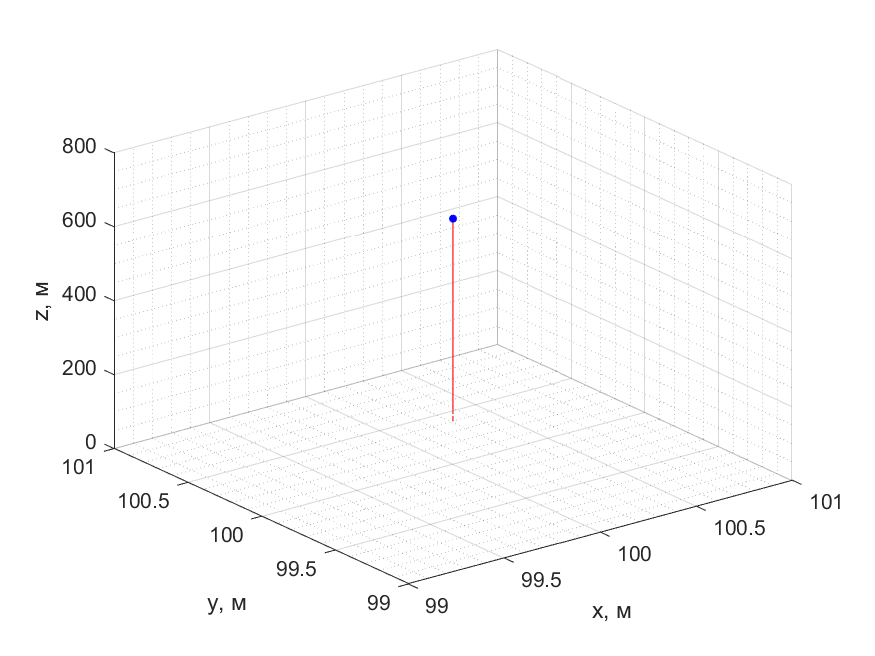
\includegraphics[width=0.75 \textwidth]{modeling_v_0_1_1.png}
    \caption{График моделирования квадрокоптера при входных напряжениях: \(U_1=5.5\)В, \(U_2=5.5\)В, \(U_3=5.5\)В, \(U_4=5.5\)В. Внешнее сопротивление отсутствует.}
    \label{fig:modeling-1}
\end{figure}

\begin{figure}[ht]
    \centering
    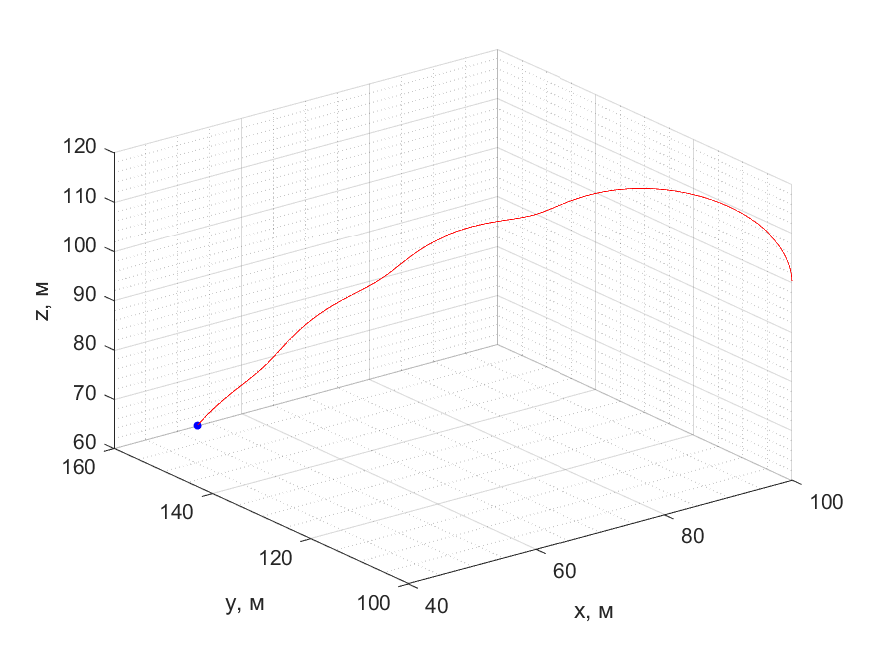
\includegraphics[width=0.75 \textwidth]{modeling_v_0_1_2.png}
    \caption{График моделирования квадрокоптера при входных напряжениях: \(U_1=5.5\)В, \(U_2=5.5\)В, \(U_3=0\)В, \(U_4=0\)В. Внешнее сопротивление отсутствует.}
    \label{fig:modeling-2}
\end{figure}

\begin{figure}[ht]
    \centering
    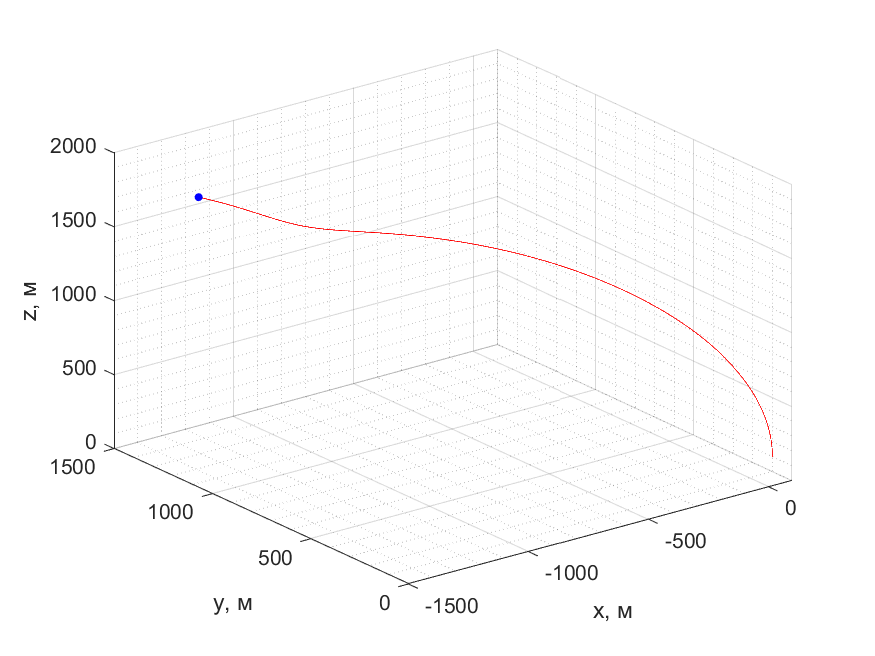
\includegraphics[width=0.8 \textwidth]{modeling_v_0_1_3.png}
    \caption{График моделирования квадрокоптера при входных напряжениях: \(U_1=5.5\)В, \(U_2=5.5\)В, \(U_3=5.4\)В, \(U_4=5.4\)В. Внешнее сопротивление отсутствует.}
    \label{fig:modeling-3}
\end{figure}

\begin{figure}[ht]
    \centering
    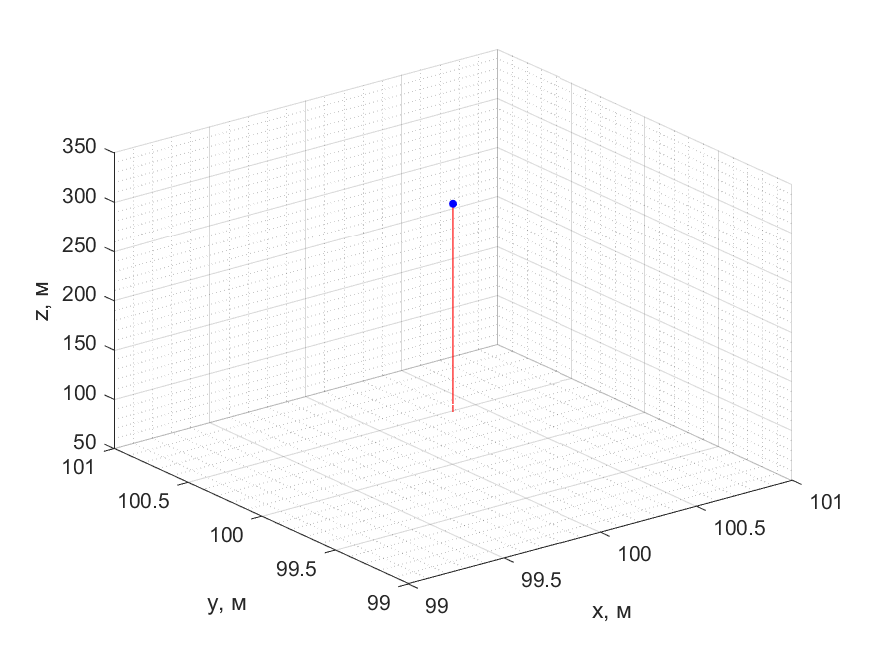
\includegraphics[width=0.8 \textwidth]{modeling_v_0_1_4.png}
    \caption{График моделирования квадрокоптера при входных напряжениях: \(U_1=5.5\)В, \(U_2=5.5\)В, \(U_3=5.5\)В, \(U_4=5.5\)В. Коэффициенты внешних сопротивлений \(C_a=C_b=0.1\), \(C_{drag}=1.1\).}
    \label{fig:modeling-4}
\end{figure}

\begin{figure}[ht]
    \centering
    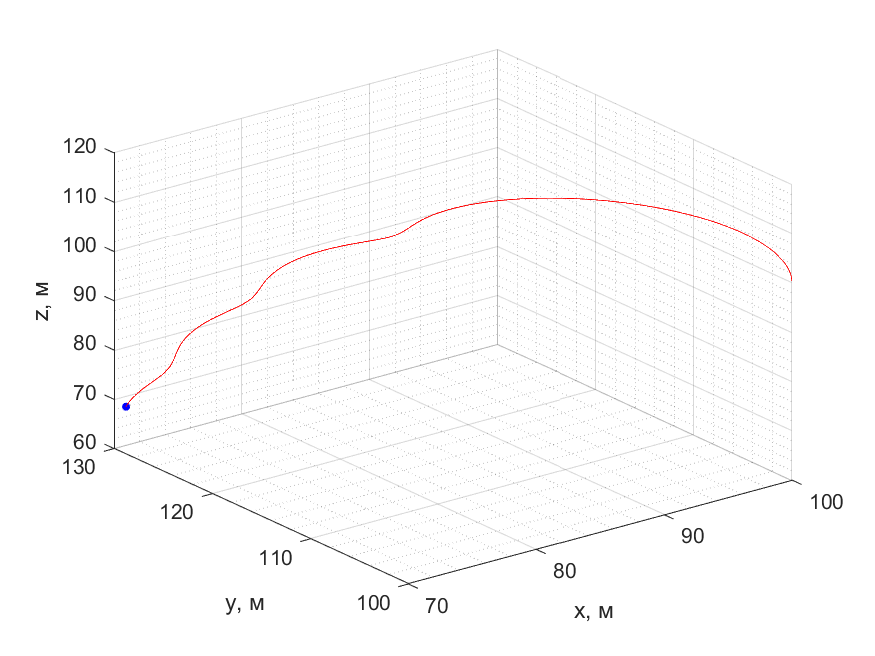
\includegraphics[width=0.8 \textwidth]{modeling_v_0_1_5.png}
    \caption{График моделирования квадрокоптера при входных напряжениях: \(U_1=5.5\)В, \(U_2=5.5\)В, \(U_3=0\)В, \(U_4=0\)В. Коэффициенты внешних сопротивлений \(C_a=C_b=0.1\), \(C_{drag}=1.1\).}
    \label{fig:modeling-5}
\end{figure}


\begin{figure}[ht]
    \centering
    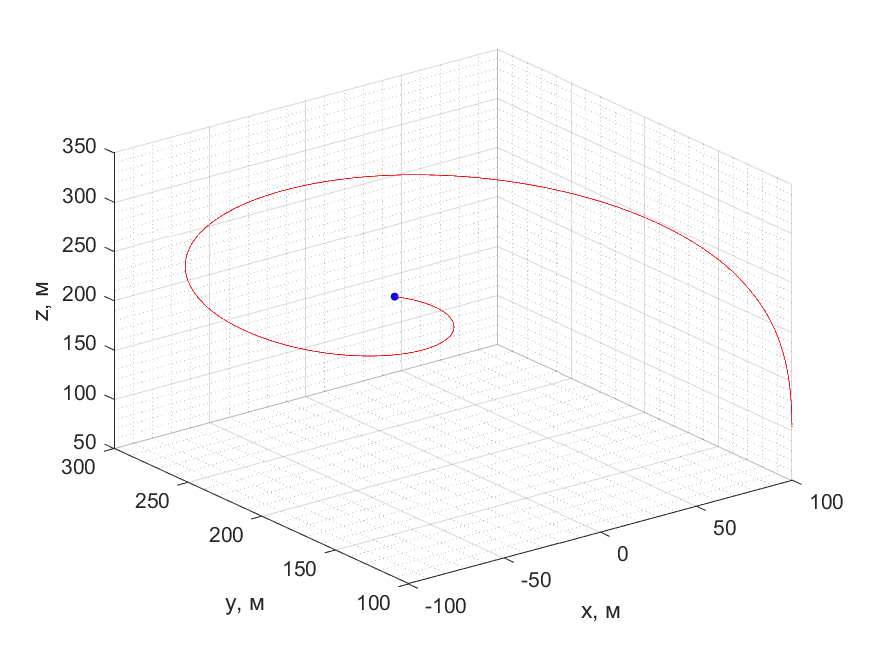
\includegraphics[width=0.8 \textwidth]{modeling_v_0_1_6.png}
    \caption{График моделирования квадрокоптера при входных напряжениях: \(U_1=5.5\)В, \(U_2=5.5\)В, \(U_3=5.4\)В, \(U_4=5.4\)В. Коэффициенты внешних сопротивлений \(C_a=C_b=0.1\), \(C_{drag}=1.1\).}
    \label{fig:modeling-6}
\end{figure}


\section{Моделирование в САПР Solidworks}

Также была создана модель квадрокоптера в САПР Solidworks.
Многие компоненты модели были найдены в интернете в свободном
доступе. В дальнейшем планируется добавить САПР модель
квадрокоптера в Simulink для более точного и наглядного 
моделирования.

\subsection{Фотографии квадрокоптера}

\begin{figure}[ht]
    \centering
    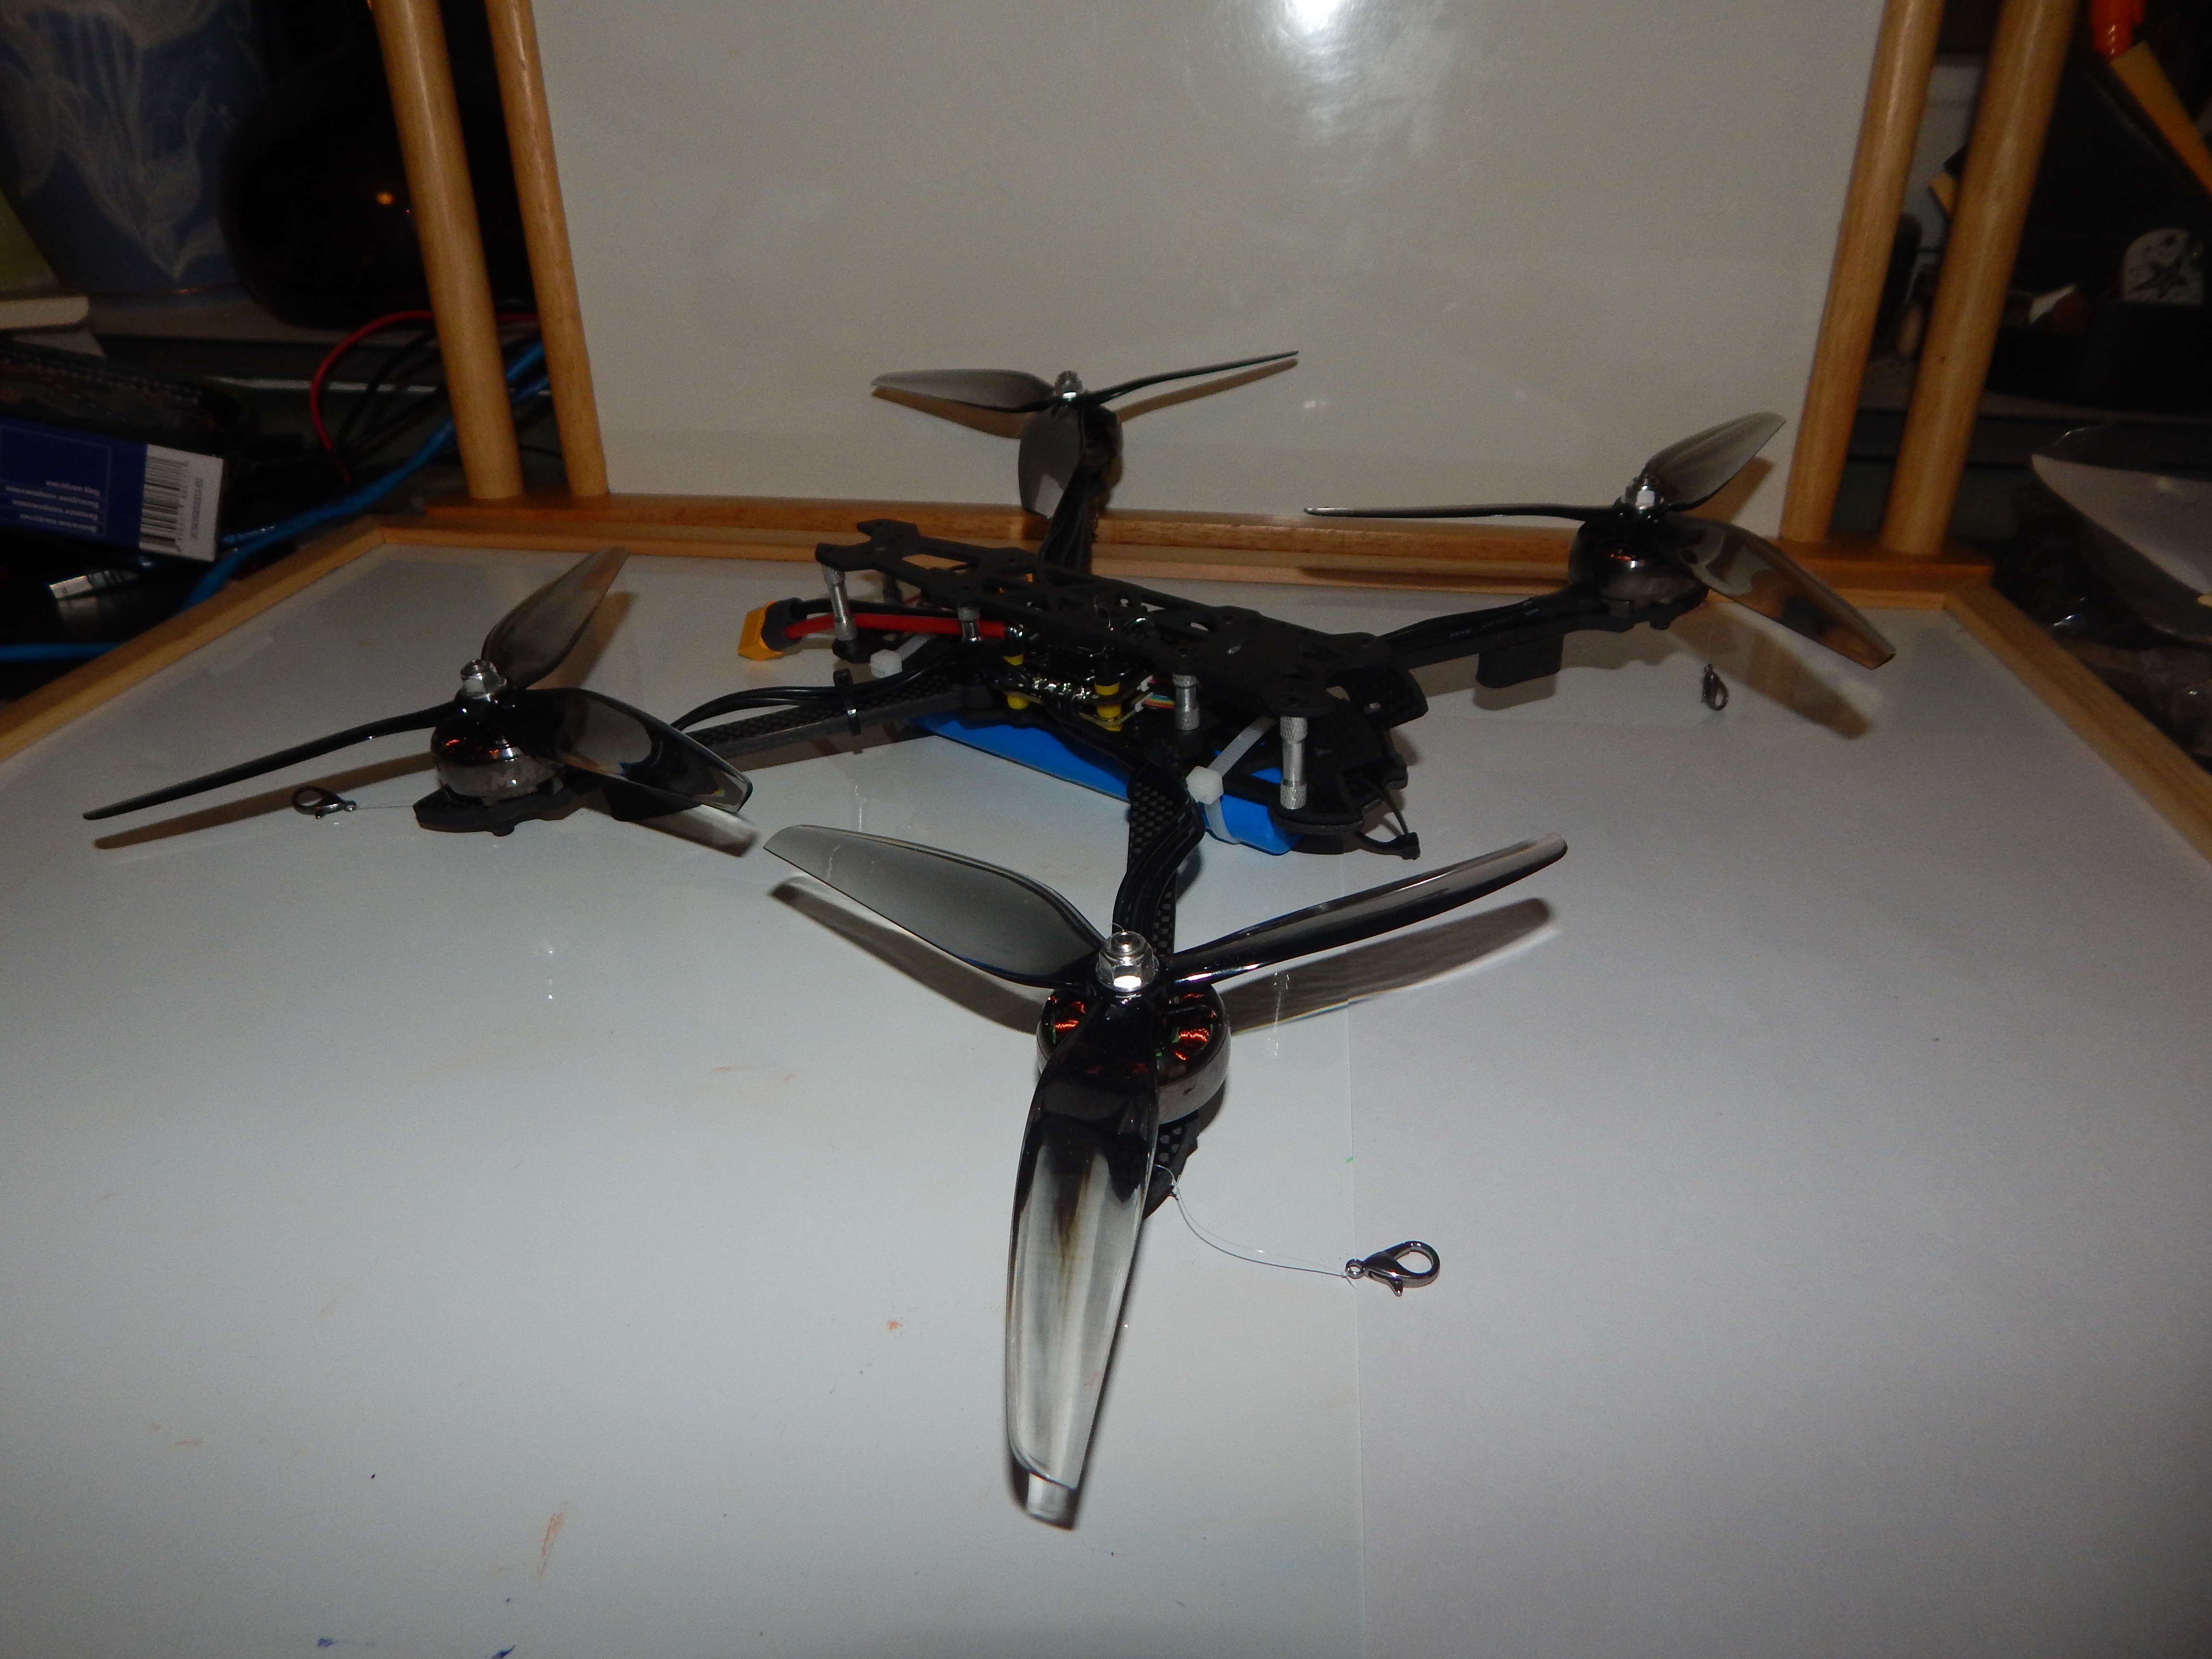
\includegraphics[width=0.8 \textwidth]{DSCN0425.JPG}
    \caption{Фотография квадрокоптера}
    \label{}
\end{figure}

\newpage

\subsection{Модель САПР}

\begin{figure}[ht]
    \centering
    \includegraphics[width=0.8 \textwidth]{cad-model-1.png}
    \caption{Модель квадрокоптера в Solidworks}
    \label{}
\end{figure}


\endinput                                     % Первая глава
% \chapter{}
\label{ch:chap1}

\section{Условие задания}
\label{sec:cond1}

\section{Расчеты}
\label{sec:calc1}

\endinput                                     % Вторая глава
% \chapter{Разработка алгоритмов управления}
\label{ch:chap2}

\section{LQR регулятор по линеаризованной модели}

В качестве одного из базовых регуляторов можно использовать LQR регулятор по линеаризованной модели.
Для синтеза регулятора определим модель системы в форме вход-состояние-выход. 

Необходимо осуществлять управление по координатам \(r_x\), \(r_y\), \(r_z\) в соответствии с этим вектор
выхода системы будет выглядеть следующим образом:

\begin{equation}
Y = \begin{bmatrix}
    r_x \\
    r_y \\
    r_z
\end{bmatrix}.
\end{equation}


Система \eqref{eq:system} в матричном виде вход-состояние-выход будет выглядеть следующим образом:


\begin{equation}
    \begin{cases}
        \dot{X} = A X + B U + D;\\
        Y = C X.
    \end{cases}
\end{equation}


Вектор состояния расширен, добавлением положением по координатам \(r_x\), \(r_y\) и \(r_z\).

\begin{equation}
X = \begin{bmatrix} 
    r_x & 
    r_y & 
    r_z & 
    \dot{r}_x & 
    \dot{r}_y & 
    \dot{r}_z & 
    \phi &
    \theta & 
    \psi &
    \omega_{\phi} & 
    \omega_{\theta} & 
    \omega_{\psi} 
\end{bmatrix}^T.
\end{equation}

Вектор управления:

\begin{equation}
U = \begin{bmatrix}
    T \\
    \tau_\phi \\
    \tau_\theta \\
    \tau_\psi
\end{bmatrix}.
\end{equation}

\newpage
Матрица \(A\) будет выглядеть следующим образом:

\begin{equation}
    A=
\begin{bmatrix}
    0 & 0 & 0 & 1 & 0 & 0 & 0 & 0 & 0 & 0 & 0 & 0 \\
    0 & 0 & 0 & 0 & 1 & 0 & 0 & 0 & 0 & 0 & 0 & 0 \\
    0 & 0 & 0 & 0 & 0 & 1 & 0 & 0 & 0 & 0 & 0 & 0 \\
    0 & 0 & 0 & A_{drag_{1:1}} & A_{drag_{1:2}} & A_{drag_{1:3}} & 0 & 0 & 0 & 0 & 0 & 0 \\
    0 & 0 & 0 & A_{drag_{2:1}} & A_{drag_{2:2}} & A_{drag_{2:3}} & 0 & 0 & 0 & 0 & 0 & 0 \\
    0 & 0 & 0 & A_{drag_{3:1}} & A_{drag_{3:2}} & A_{drag_{3:3}} & 0 & 0 & 0 & 0 & 0 & 0 \\
    0 & 0 & 0 & 0 & 0 & 0 & 1 & T_\theta S_\phi & T_\theta C_\phi & 0 & 0 & 0 \\
    0 & 0 & 0 & 0 & 0 & 0 & 0 & C_\phi & -S_\phi & 0 & 0 & 0 \\
    0 & 0 & 0 & 0 & 0 & 0 & 0 & \frac{S_\phi}{C_\theta} & \frac{C_\phi}{C_\theta} & 0 & 0 & 0 \\
    0 & 0 & 0 & 0 & 0 & 0 & 0 & 0 & 0 & 0 & 0 & \frac{(I_z - I_y)\omega_{\theta}}{I_x} \\
    0 & 0 & 0 & 0 & 0 & 0 & 0 & 0 & 0 & 0 & 0 & \frac{(I_x - I_z)\omega_{\phi}}{I_y} \\
    0 & 0 & 0 & 0 & 0 & 0 & 0 & 0 & 0 & 0 & \frac{(I_y - I_x)\omega_{\phi}}{I_z} & 0
\end{bmatrix},
\end{equation}


где \(C_\phi = \cos\phi\), \(S_\phi = \sin\phi\), \(C_\theta = \cos\theta\), \(S_\theta = \sin\theta\),
\(T_\theta = \tan\theta\), матрица \(A_{drag}\):

\begin{equation}
A_{drag} = -\frac{T}{m} R (A_{ind} + A_{flap}) R^T - \frac{\rho C_{drag} S}{2m} \|\dot{r}\| I
.\end{equation}

Матрица \(B\):

\begin{equation}
B = \begin{bmatrix}
    0 & 0 & 0 & 0 \\
    0 & 0 & 0 & 0 \\
    0 & 0 & 0 & 0 \\
    \frac{\cos \psi \sin \theta \cos \phi + \sin \psi \sin \phi}{m} & 0 & 0 & 0 \\
    \frac{\sin \psi \sin \theta \cos \phi - \cos \psi \sin \phi}{m} & 0 & 0 & 0 \\
    \frac{\cos\theta\cos\phi}{m} & 0 & 0 & 0 \\
    0 & 0 & 0 & 0 \\
    0 & 0 & 0 & 0 \\
    0 & 0 & 0 & 0 \\
    0 & \frac{1}{I_x} & 0 & 0 \\
    0 & 0 & \frac{1}{I_y} & 0 \\
    0 & 0 & 0 & \frac{1}{I_z} \\
    \end{bmatrix}.
\end{equation}

\newpage

Матрица \(D\)

\begin{equation}
D = \begin{bmatrix}
    0 & 0 & 0 & 0 & 0 & -g & 0 & 0 & 0 & 0 & 0 & 0 \\
\end{bmatrix}^T.
\end{equation}

Матрица \(C\):

\begin{equation}
C = \begin{bmatrix}
    1 & 0 & 0 & 0 & 0 & 0 & 0 & 0 & 0 & 0 & 0 & 0 \\
    0 & 1 & 0 & 0 & 0 & 0 & 0 & 0 & 0 & 0 & 0 & 0 \\
    0 & 0 & 1 & 0 & 0 & 0 & 0 & 0 & 0 & 0 & 0 & 0 
\end{bmatrix}.
\end{equation}

\subsection{Линеаризация у точки равновесия}

Для синтеза LQR регулятора необходимо сначала линеаризовать квадрокоптер.

Производится линеаризация около точки равновесия, в которой угловые 
скорости и ускорения равны нулю. Состояние системы, которое будет соответствовать точке 
равновесия будет определяться следующим образом:

\begin{equation}
    \bar{X} = \begin{bmatrix}
        \bar{r}_x & \bar{r}_y & \bar{r}_z & 0 & 0 & 0 & 0 & 0 & \psi & 0 & 0 & 0 
    \end{bmatrix}.
    \label{eq:point1}
\end{equation}

Линеаризация системы у точки \eqref{eq:point1}:


\begin{equation}
    \bar{A} = 
    \begin{bmatrix}
    0 & 0 & 0 & 1 & 0 & 0 & 0 & 0 & 0 & 0 & 0 & 0 \\
    0 & 0 & 0 & 0 & 1 & 0 & 0 & 0 & 0 & 0 & 0 & 0 \\
    0 & 0 & 0 & 0 & 0 & 1 & 0 & 0 & 0 & 0 & 0 & 0 \\
    0 & 0 & 0 & \bar{A}_{drag_{1:1}} & \bar{A}_{drag_{1:2}} & \bar{A}_{drag_{1:3}} & 0 & 0 & 0 & 0 & 0 & 0 \\
    0 & 0 & 0 & \bar{A}_{drag_{2:1}} & \bar{A}_{drag_{2:2}} & \bar{A}_{drag_{2:3}} & 0 & 0 & 0 & 0 & 0 & 0 \\
    0 & 0 & 0 & \bar{A}_{drag_{3:1}} & \bar{A}_{drag_{3:2}} & \bar{A}_{drag_{3:3}} & 0 & 0 & 0 & 0 & 0 & 0 \\
    0 & 0 & 0 & 0 & 0 & 0 & 1 & 0 & 0 & 0 & 0 & 0 \\
    0 & 0 & 0 & 0 & 0 & 0 & 0 & 1 & 0 & 0 & 0 & 0 \\
    0 & 0 & 0 & 0 & 0 & 0 & 0 & 0 & 1 & 0 & 0 & 0 \\
    0 & 0 & 0 & 0 & 0 & 0 & 0 & 0 & 0 & 0 & 0 & 0 \\
    0 & 0 & 0 & 0 & 0 & 0 & 0 & 0 & 0 & 0 & 0 & 0 \\
    0 & 0 & 0 & 0 & 0 & 0 & 0 & 0 & 0 & 0 & 0 & 0
\end{bmatrix},
\end{equation}

где  

\begin{equation}
    \bar{A}_{drag} = - \frac{T}{m} (A_{ind} + A_{flap});
\end{equation}


\begin{equation}
    \bar{B} = \begin{bmatrix}
    0 & 0 & 0 & 0 \\
    0 & 0 & 0 & 0 \\
    0 & 0 & 0 & 0 \\
    0 & 0 & 0 & 0 \\
    0 & 0 & 0 & 0 \\
    \frac{1}{m} & 0 & 0 & 0 \\
    0 & 0 & 0 & 0 \\
    0 & 0 & 0 & 0 \\
    0 & 0 & 0 & 0 \\
    0 & \frac{1}{I_x} & 0 & 0 \\
    0 & 0 & \frac{1}{I_y} & 0 \\
    0 & 0 & 0 & \frac{1}{I_z} \\
    \end{bmatrix}.
\end{equation}

Матрицы \(C\) и \(D\) остаются без изменений.

LQR регулятор минимизирует критерий качества, который определяется как:

\begin{equation}
    J = \int_0^\infty \left( X^T Q X + U^T R U \right) dt.
\end{equation}

Для синтеза LQR регулятора необходимо определить матрицы \(Q\) и \(R\), которые определяют весовые коэффициенты для состояния и 
управления соответственно.
Пусть \(Q\) и \(R\) будут определены следующим образом:

\[
    Q = \begin{bmatrix}
        10 & 0 & 0 & 0 & 0 & 0 & 0 & 0 & 0 & 0 & 0 & 0 \\ %1
        0 & 10 & 0 & 0 & 0 & 0 & 0 & 0 & 0 & 0 & 0 & 0 \\ %2
        0 & 0 & 30 & 0 & 0 & 0 & 0 & 0 & 0 & 0 & 0 & 0 \\ %3
        0 & 0 & 0 & 0 & 0 & 0 & 0 & 0 & 0 & 0 & 0 & 0 \\ %4
        0 & 0 & 0 & 0 & 0 & 0 & 0 & 0 & 0 & 0 & 0 & 0 \\ %5
        0 & 0 & 0 & 0 & 0 & 0 & 0 & 0 & 0 & 0 & 0 & 0 \\ %6
        0 & 0 & 0 & 0 & 0 & 0 & 10 & 0 & 0 & 0 & 0 & 0 \\ %7
        0 & 0 & 0 & 0 & 0 & 0 & 0 & 10 & 0 & 0 & 0 & 0 \\ %8
        0 & 0 & 0 & 0 & 0 & 0 & 0 & 0 & 10 & 0 & 0 & 0 \\ %9
        0 & 0 & 0 & 0 & 0 & 0 & 0 & 0 & 0 & 0 & 0 & 0 \\    %10
        0 & 0 & 0 & 0 & 0 & 0 & 0 & 0 & 0 & 0 & 0 & 0 \\    %11
        0 & 0 & 0 & 0 & 0 & 0 & 0 & 0 & 0 & 0 & 0 & 0 \\    %12
    \end{bmatrix};
\]

\[
    R = \begin{bmatrix}
        1 & 0 & 0 & 0  \\ %1
        0 & 1 & 0 & 0 \\ %2
        0 & 0 & 1 & 0  \\ %3
        0 & 0 & 0 & 1
    \end{bmatrix}.
\]


Для обеспечения минимизации критерия качества \(J\) используется решение уравнения Риккати:

\begin{equation} 
    A^T P + P A - P B R^{-1} B^T P + Q = 0.
\end{equation}

Из этого уравнения можно получить \(P\) — матрица, с помощью которой можно найти матрицу \(K\) для LQR регулятора:

\begin{equation}
    K = R^{-1} B^T P.
\end{equation} 

Управление в системе будет осуществляться по следующему закону:
\begin{equation}
    U = -K X.
\end{equation}

Рассчитанные коэффициенты:

\[
    K =\begin{bmatrix}
        0 & 0 & 5.48 & 0 & 0 & 2.67 & 0 & 0 & 0 & 0 & 0 & 0 \\
        0 & -3.16 & 0 & 0 & -1.54 & 0 & 3.69 & 0 & 0 & 0.13 & 0 & 0 \\
        3.16 & 0 & 0 & 1.54 & 0 & 0 & 0 & 3.69 & 0 & 0 & 0.13 & 0 \\
        0 & 0 & 0 & 0 & 0 & 0 & 0 & 0 & 3.16 & 0 & 0 & 0.17
        \end{bmatrix}.
\]


\section{LQR регулятор с линеаризацией обратной связью}

В линеаризации обратной связью необходимо упростить уравнения квадрокоптера вводом 
новых виртуальных управлений. Управления будут выглядеть следующим образом:

% Без сопротивлений

\begin{equation}
    \begin{cases}
        \nu_x = \frac{1}{m} (\cos\phi \sin\theta  + \sin\psi \sin\phi) U_1;\\
        \nu_y = \frac{1}{m} (\sin\psi \sin\theta \cos\phi - \cos\psi \sin\phi) U_1;\\
        \nu_z = -g + \frac{1}{m} \cos\theta \cos\phi U_1;\\
        \nu_\phi = \frac{I_z - I_y}{I_x}\omega_\psi \omega_\theta + \frac{1}{I_x} U_2;\\
        \nu_\theta = \frac{I_x - I_z}{I_y}\omega_\phi \omega_\psi + \frac{1}{I_y} U_2;\\
        \nu_\psi = \frac{I_y - I_x}{I_z}\omega_\phi \omega_\theta + \frac{1}{I_z} U_2.
    \end{cases}
\end{equation}

Введение ошибок состояния:

\begin{equation}
\begin{aligned}
&\tilde{r}_x = r_x - r_x^d; \quad \tilde{v}_x = v_x - v_x^d; \\
&\tilde{r}_y = r_y - r_y^d; \quad \tilde{v}_y = v_y - v_y^d; \\
&\tilde{r}_z = r_z - r_z^d; \quad \tilde{v}_z = v_z - v_z^d; \\
&\tilde{\phi} = \phi - \phi^d; \quad \tilde{\omega}_\phi = \omega_\phi - \omega_\phi^d; \\
&\tilde{\theta} = \theta - \theta^d; \quad \tilde{\omega}_\theta = \omega_\theta - \omega_\theta^d; \\
&\tilde{\psi} = \psi - \psi^d; \quad \tilde{\omega}_\psi = \omega_\psi - \omega_\psi^d.
\end{aligned}
\end{equation}  

Динамика ошибок преобразуется в линейные подсистемы:  
\begin{equation}
\begin{cases} 
\dot{\tilde{r}}_x = \tilde{v}_x; \\
\dot{\tilde{v}}_x = \nu_x;
\end{cases}
\quad
\begin{cases} 
\dot{\tilde{r}}_y = \tilde{v}_y; \\
\dot{\tilde{v}}_y = \nu_y;
\end{cases}
\quad
\begin{cases} 
\dot{\tilde{r}}_z = \tilde{v}_z; \\
\dot{\tilde{v}}_z = \nu_z;
\end{cases}
\end{equation}
 
\begin{equation}
\begin{cases} 
\dot{\tilde{\phi}} = \tilde{\omega}_\phi; \\
\dot{\tilde{\omega}}_\phi = \nu_\phi;
\end{cases}
\quad
\begin{cases} 
\dot{\tilde{\theta}} = \tilde{\omega}_\theta; \\
\dot{\tilde{\omega}}_\theta = \nu_\theta;
\end{cases}
\quad
\begin{cases} 
\dot{\tilde{\psi}} = \tilde{\omega}_\psi; \\
\dot{\tilde{\omega}}_\psi = \nu_\psi.
\end{cases}
\end{equation}


Для каждой подсистемы применяется LQR регулятор:

\begin{equation}
    \begin{cases}
    \nu_x = -k_1^x \tilde{r}_x - k_2^x \tilde{v}_x; \\
    \nu_y = -k_1^y \tilde{r}_y - k_2^y \tilde{v}_y; \\
    \nu_z = -k_1^z \tilde{r}_z - k_2^z \tilde{v}_z; \\
    \nu_\phi = -k_1^\phi \tilde{\phi} - k_2^\phi \tilde{\omega}_\phi; \\
    \nu_\theta = -k_1^\theta \tilde{\theta} - k_2^\theta \tilde{\omega}_\theta; \\
    \nu_\psi = -k_1^\psi \tilde{\psi} - k_2^\psi \tilde{\omega}_\psi.
    \end{cases}
\end{equation}

Для подсистеме по координате \(r_x\) синтез LQR регулятор выглядит следующим образом:
Матрицы состояния и управления:

\begin{equation}
    A_x=\begin{bmatrix}
    0 & 1 \\
    0 & 0
\end{bmatrix}, \quad
B_x = \begin{bmatrix}
    0 \\
    1
\end{bmatrix}.\end{equation}

Осуществляется выбор матриц \(Q\) и \(R\) для критерия качества. 
И решается уравнение Риккати:

\begin{equation}
    A_x^T P + P A_x - P B_x R^{-1} B_x^T P + Q = 0.
\end{equation}

Откуда получаем коэффициенты \(k_1^x\) и \(k_2^x\):
\begin{equation}
    k^x = R^{-1} B_x^T P.
\end{equation}

Аналогично синтезируются регуляторы для остальных подсистем.

Полученные виртуальные управления обратно преобразуются в реальные управления:

\begin{equation}
    \begin{cases}
        \bar{\phi} = \frac{v_x}{v_z+g};\\
        \bar{\theta} =  \frac{v_y}{v_z+g};
    \end{cases}
\end{equation}

\begin{equation}
    \begin{cases}
    U_1 = \frac{m (\nu_z + g)}{\cos\bar{\phi} \cos\bar{\theta}}; \\
    U_2 = I_x \nu_\phi - (I_y - I_z) \omega_\theta \omega_\psi; \\
    U_2 = I_y \nu_\theta - (I_x - I_z) \omega_\phi \omega_\psi; \\
    U_4 = I_z \nu_\psi - (I_x - I_y) \omega_\phi \omega_\theta.
    \end{cases}
\end{equation}
% С сопротивлениями
Для управлений были выбраны различные матрицы \(Q\) и \(R\), полученные коэффициенты регулятора:

\[
K = \begin{bmatrix}
    5  & 5  &  3  & 141 & 141 & 0 \\
    10 & 10 &  3  & 1000 & 1000 & 0 
\end{bmatrix}^T.
\]


\section{Nonlinear MPC}

Nonlinear MPC --- один из самых эффективных регуляторов с точки зрения оптимизации управления и 
точности. Суть регулятора довольно простая, на вход поступает вектор состояний квадрокоптера 
и желаемое состояние на некоторое количество 
шагов вперед. Количество шагов называется горизонтом предсказания. Далее 
внутри регулятора происходит моделирование поведение квадрокоптера с управлением, которое может быть
изначально проинициализировано или получено с предыдущего шага.
Затем происходит минимизация заданного критерия качества, который обычно имеет следующий вид:

\begin{equation}
    J = \sum_{k=0}^{N-1} \left( e_k^T Q e_k + u_k^T R u_k \right),
\end{equation}

где \(X_k\) — состояние системы на \(k\)-м шаге, \(X_k^d\) — желаемое состояние на \(k\)-м шаге, \(U_k\) — управление на \(k\)-м шаге, \(Q\) и \(R\) — весовые матрицы, определяющие важность отклонения состояния и управления соответственно, \(N\) — горизонт предсказания.

Минимизация критерия качества осуществляется с учетом ограничений на динамику системы, которые задаются в виде:

\begin{equation}
    X_{k+1} = f(X_k, U_k),
\end{equation}

где \(f(X_k, U_k)\) — нелинейная модель квадрокоптера, а также ограничений на управление и состояния, например:

\begin{equation}
    U_{\text{min}} \leq U_k \leq U_{\text{max}}, \quad X_{\text{min}} \leq X_k \leq X_{\text{max}}.
\end{equation}

Решение задачи оптимизации дает последовательность управлений \(\{U_0, U_1, \dots, U_{N-1}\}\), из которых на выходе регулятора используется только первое управление \(U_0\). Это управление подается на квадрокоптер, после чего процесс повторяется на следующем временном шаге с обновленным состоянием системы.


Регулятор можно расширять и модифицировать, можно ввести ограничения, штрафные стоимости за быстрые переключения управления,
изменить модель объекта, например учитывать характер внешних возмущений.


В среде Matlab/Simulink есть реализация Nonlinear MPC регулятора, но в текущей работе было принято решение полностью написать 
функцию Nonlinear MPC регулятора с введением некоторых модификаций, и чтобы в дальнейшем было проще перенести 
реализацию на реальную систему.

Система управления не разделена на контуры, 
и реализует вышеописанную логику. Схема регулятора представлена на рисунке \ref{fig:mpc-1}. 
Для минимизации критерия \(J\) используется градиентный спуск, в математическом представлении:

\begin{equation}
    U_{k+1} = U_k - \nabla J(U_k).
\end{equation}

Также введены дополнительные мягкие ограничения на углы \(\phi\) и \(\theta\), чтобы квадрокоптер
не переворачивался в воздухе.

\begin{figure}[ht]
    \centering
    \includegraphics[width=0.8 \textwidth]{mpc-1.png}
    \caption{Схема регулятора Nonlinear MPC}
    \label{fig:mpc-1}
\end{figure}


\endinput                                     % Третья глава
% \chapter{}
\label{ch:chap3}

\section{}
\label{sec:cond3}


\endinput     
% \chapter{Реализация квадрокоптера на базе STM32F722}

Основной задачей являлась 
реализация эффективной системы стабилизации и управления 
полетом с использованием линейного квадратичного регулятора LQR 
с линеаризацией обратной связью. Выбор 
LQR был обусловлен его хорошим соотношением между вычислительной 
нагрузкой и качеством управления, что видно 
по результатам моделирования приведенным в предыдущей главе.

\section{Аппаратная часть квадрокоптера}

В результате разработан квадрокоптер, построенный на базе готового 
полетного контроллера Radiolink F722, в основе которого лежит 
микроконтроллер STM32F722\cite{RadiolinkF722}\cite{STM32F722}. 
Полетный контроллер Radiolink F722 включает в себя встроенный датчик пространственного положения 
и гироскопа ICM42688-P. Взаимодействие с датчиком осуществлялось по интерфейсу SPI\cite{ICM42688P}.


\begin{figure}[ht]
    \centering
    \includegraphics[width=0.3 \textwidth]{flight-controller-1.png}
    \caption{Полетный контроллер Radiolink F722}
    \label{}
\end{figure}

Управление четырьмя моторами осуществлялось с помощью широтно-импульсной модуляции
через электронные регуляторы скорости(ESC). На квадрокоптер были установлены популярные бесколлектрные моторы
EMAX ECO || 2306 1300 KV\cite{EmaxECO1300KV}. KV --- это стандартная характеристика бесколлекторных моторов, которое означает
количество оборотов на вольт без нагрузки.

\begin{figure}[ht]
    \centering
    \includegraphics[width=0.45 \textwidth]{motor-1.png}
    \caption{Мотор EMAX ECO || 2306 1300 KV}
    \label{}
\end{figure}


В качестве рамы квадрокоптера было выбрано готовое решение --- корпус Mark 4 295 мм.

\begin{figure}[ht]
	\centering
	\includegraphics[width=0.8 \textwidth]{drone.JPG}
	\caption{Квадрокоптер в собранном виде}
	\label{}
\end{figure}


В среде САПР среде Solidworks была реализована 3D модель квадрокоптера. Эта модель была
импортирована в среду Matlab/Simulink для имитационного моделирования.

\begin{figure}[ht]
	\centering
	\includegraphics[width=0.8 \textwidth]{cad-model-1.png}
	\caption{3D модель квадрокоптера в Solidworks}
	\label{}
\end{figure}

\section{Программное обеспечение квадрокоптера}

Разработка программного обеспечения велась в среде 
STM32CubeIDE. Предварительно были изучены исходные файлы открытой 
прошивки полетных контроллеров Betaflight, благодаря которым удалось произвести
обратное проектирование полетного контроллера для разработки собственного программного обеспечения\cite{Betaflight}.

Для удобной и универсальной коммуникации с квадрокоптером была выбрана коммуникация по 
протоколу MQTT, который часто используется в проектах интернет вещей в сетях 
с низкой пропускной способностью\cite{MQTT}. Таким образом сообщения доходят быстро и довольно стабильно
при должной настройке. Так как микроконтроллер STM32F722 не оснащен WI-FI модулем к нему 
был подключен микроконтроллер ESP8266, который обладает встроенным WI-FI модулем и способен 
принимать команды по MQTT, передавая их на STM32F722 по интерфейсу UART.

\begin{figure}[ht]
	\centering
\hspace*{\fill}%
	\begin{subfigure}[b]{0.49\textwidth}
        \centering
		\includegraphics[height=9cm,keepaspectratio]{esp8266.png}
		\caption{}
		\label{fig:tiger1}
	\end{subfigure}
\hfill
	\begin{subfigure}[b]{0.49\textwidth}
        \centering
		\includegraphics[height=9cm,keepaspectratio]{drone-inside-1.png}
        \caption{}
		\label{fig:tiger2}
	\end{subfigure}
\hspace*{\fill}%
	\caption{На рисунке (а) ESP8266. На рисунке (б)Встроенный ESP8266 на квадрокоптере}
	\label{fig:tiger}
\end{figure}

\newpage

Также был сделана панель управления для управления квадрокоптером через окно
браузера. 


\begin{figure}[ht]
	\centering
\hspace*{\fill}%
	\begin{subfigure}[b]{0.49\textwidth}
        \centering
		\includegraphics[height=9cm,keepaspectratio]{dashboard-1.png}
		\caption{}
		\label{fig:tiger1}
	\end{subfigure}
\hfill
	\begin{subfigure}[b]{0.49\textwidth}
        \centering
		\includegraphics[height=9cm,keepaspectratio]{dashboard-2.png}
        \caption{}
		\label{fig:tiger2}
	\end{subfigure}
\hspace*{\fill}%
	\caption{Панель управления квадрокоптером в браузере}
	\label{fig:tiger}
\end{figure}

В качестве брокера сообщений для обеспечения передачи команд от компьютера к 
микроконтроллеру ESP8266 был выбран популярный - Mosquitto, который можно развернуть 
локальной машине\cite{Mosquitto}.

\newpage

\section{Локализация квадрокоптера}

Для решения задачи локализации квадрокоптера было решено использовать визуальные маркеры apriltag\cite{AprilTag}.
В библиотеке OpenCV уже есть встроенные функции для детектирования и отслеживания маркеров apriltag\cite{OpenCV}\cite{Aruco}.
Были также написана логика для калибровки камеры для получения координат 
 по осям: X, Y, Z в системе СИ. Код приложения для отслеживания визуального маркера 
запускался на одноплатном компьютере Raspberry PI 4b с 4 Гб оперативной памяти. 
Использовалась камера Raspberry Pi Camera Module Rev 1.3 с разрешением 5 мегапикселей.
На каждом кадре осуществляется поиск маркера, рассчитанные координаты отправляются по
MQTT на квадрокоптер.


\begin{figure}[ht]
    \centering
    \includegraphics[width=0.5 \textwidth]{drone-apriltag.png}
    \caption{Apriltag 36h11 закрепленный на квадрокоптере}
    \label{}
\end{figure}

\begin{figure}[ht]
	\centering
\hspace*{\fill}%
	\begin{subfigure}[b]{0.49\textwidth}
        \centering
		\includegraphics[height=9cm,keepaspectratio]{camera+drone_1.png}
		\caption{}
		\label{fig:tiger1}
	\end{subfigure}
\hfill
	\begin{subfigure}[b]{0.49\textwidth}
        \centering
		\includegraphics[height=9cm,keepaspectratio]{camera+drone_2.png}
        \caption{}
		\label{fig:tiger2}
	\end{subfigure}
\hspace*{\fill}%
	\caption{Детектирование тэга на камере}
	\label{fig:tiger}
\end{figure}

\newpage


\section{Тестирование квадрокоптера}

Разработанный прототип частично тестировался в полевых условиях на двух стендах и в свободном полете.


\begin{figure}[ht]
    \centering
    \includegraphics[width=0.5 \textwidth]{drone_fly_1.png}
    \caption{Тестирование квадрокоптера в свободном полете}
    \label{}
\end{figure}

\begin{figure}[ht]
	\centering
\hspace*{\fill}%
	\begin{subfigure}[b]{0.49\textwidth}
        \centering
		\includegraphics[height=9cm,keepaspectratio]{test-2.png}
		\caption{}
		\label{fig:tiger1}
	\end{subfigure}
\hfill
	\begin{subfigure}[b]{0.49\textwidth}
        \centering
		\includegraphics[height=9cm,keepaspectratio]{test-1.png}
        \caption{}
		\label{fig:tiger2}
	\end{subfigure}
\hspace*{\fill}%
	\caption{Тестирование квадрокоптера на стендах}
	\label{fig:tiger}
\end{figure}

Тестирование на предмет слежения за траекторией не удалось в силу трудностей с построением специального полигона, 
однако
регулятор показал свою работоспособность в решении задачи стабилизации 
квадрокоптера. 


\endinput
%\chapter*{Список использованных источников}
\addcontentsline{toc}{chapter}{Список использованных источников}



\endinput
% \chapter*{Заключение}
\addcontentsline{toc}{chapter}{Заключение}
\label{ch:chap1}

В рамках выполнения работы были достигнуты поставленные цели: 
разработаны алгоритмы управления квадрокоптером для слежения за траекторией, 
проведено их моделирование в среде MATLAB/Simulink, выполнено сравнение 
качества переходных процессов, наиболее эффективный алгоритм 
реализован на реальном квадрокоптере.

Проведённое моделирование системы управления дроном на траекториях `восьмёрка' и `куб' 
позволило оценить эффективность трёх регуляторов: классического LQR, LQR с 
линеаризацией обратной связью (LQR+FB) и нелинейного MPC. Наибольшую точность 
демонстрируют регуляторы LQR+FB и MPC. Например, для траектории «восьмёрка» 
RMSE положения по осям X и Y у MPC составили 0.463 м и 0.305 м соответственно, 
что близко к результатам LQR+FB (0.470 м и 0.324 м). При этом MPC обеспечил минимальную
 ошибку по высоте (0.501 м), что подтверждает его преимущество в условиях отсутствия возмущений.

Регулятор LQR+FB показал значительно более высокую скорость моделирования 
благодаря меньшей вычислительной сложности по сравнению с MPC. 
Но нужно отметить, что регулятор MPC обладает высокой расширяемостью и 
конфигурируемостью. Возможность 
учёта нелинейностей, ограничений на состояния и управления, 
а также адаптация к агрессивным маневрам открывают перспективы 
для дальнейшего улучшения точности. Однако его реализация 
требует значительных вычислительных ресурсов, что может ограничивать применение в реальном времени.

В связи с отмеченными недостатками MPC регулятора было решено использовать
LQR регулятор с линеаризацией обратной связью для экспериментов на реальном квадрокоптере.
В ходе разработки квадрокоптера было реализовано следующее: программное обеспечение для квадрокоптера на
базе микроконтроллера STM32F722;
система коммуникации с квадрокоптером посредством MQTT протокола и микроконтроллера ESP8266; 
панель управления для браузера; система локализации с использованием визуальных маркеров
apriltag. Было проведено тестирование регулятора для стабилизации квадрокоптера на двух стендах. 

Выбор регулятора зависит от условий задачи и располагаемых ресурсов, соответственно 
LQR с линеаризацией обратной связью
будет очень хорошим и эффективным регулятором для решения многих задач, 
но MPC будет лучшим выбором, если есть большие вычислительные мощности и временные ресурсы для 
настройки параметров и модификации регулятора. 

\endinput

\chapter*{Заключение}
\addcontentsline{toc}{chapter}{Заключение}
\label{ch:chap1}

В ходе работы была рассмотрена математическая модель динамики квадрокоптера.
Модель основана на уравнениях Ньютона-Эйлера, 
которые описывают поступательное и вращательное движение аппарата. 
Учитываются шесть степеней свободы: три линейных (X, Y, Z) 
и три угловых (крен, тангаж, рыскание).

Также была создана компьютерная модель на основании синтезированных уравнений.
Проведено компьютерное моделирование и построены графики, судя по которым 
модель вполне соответствует реальности.

Помимо математической модели была создана 3D модель квадрокоптера в системе
САПР Solidworks. Эта модель в дальнейшем будет интегрирована в 
среду Simulink.

Полученные результаты могут быть использованы для 
дальнейшей разработки системы управления квадрокоптером.

\endinput
\nocite{*}
\printbibliography[title=Список использованных источников]

\end{document}